%%%%%%%%%%%%%%%%%%%%%%%%%%%%%%%%%%%%%%%%%
% Structured General Purpose Assignment
% LaTeX Template
%
% This template has been downloaded from:
% http://www.latextemplates.com
%
% Original author:
% Ted Pavlic (http://www.tedpavlic.com)
%
% Note:
% The \lipsum[#] commands throughout this template generate dummy text
% to fill the template out. These commands should all be removed when 
% writing assignment content.
%
%%%%%%%%%%%%%%%%%%%%%%%%%%%%%%%%%%%%%%%%%

%----------------------------------------------------------------------------------------
%	PACKAGES AND OTHER DOCUMENT CONFIGURATIONS
%----------------------------------------------------------------------------------------

\documentclass[a4paper, 12pt]{article}

\usepackage{fancyhdr} % Required for custom headers
\usepackage{amsmath}
\usepackage{lastpage} % Required to determine the last page for the footer
\usepackage{extramarks} % Required for headers and footers
\usepackage{graphicx} % Required to insert images
\usepackage{indentfirst} % Required to indent the first paragraph
\usepackage[nottoc,numbib]{tocbibind} % Required to show the bibliography in the content
\usepackage[disable]{todonotes} % todo notes
\usepackage{enumitem}
\usepackage[bottom=1.2in,top=1.2in]{geometry} % Margins
\usepackage{setspace}
\usepackage{titlesec} % section title space 
\usepackage[font=small]{caption}

% Margins
% \topmargin=-0.45in
\evensidemargin=0in
\oddsidemargin=0in
\textwidth=6.5in
% \textheight=9.0in
\headheight=15pt


\linespread{1.1} % Line spacing

\titlespacing*{\section}
{0pt}{10pt}{10pt}
\titlespacing*{\subsection}
{0pt}{5pt}{10pt}

% Set up the header and footer
\pagestyle{fancy}
\lhead{} % Top left header
\chead{\hmwkClass: \hmwkTitle} % Top center header
\rhead{} % Top right header
\lfoot{} % Bottom left footer
\cfoot{} % Bottom center footer
\rfoot{Page\ \thepage\ of\ \pageref{LastPage}} % Bottom right footer
\renewcommand\headrulewidth{0.4pt} % Size of the header rule
\renewcommand\footrulewidth{0.4pt} % Size of the footer rule

% rewrite the first head style
\fancypagestyle{firststyle}
{
	\renewcommand\headrulewidth{0pt}%
	\renewcommand\footrulewidth{0pt}
   \fancyhf{}
   \fancyhead[L]{
   \noindent
	\begin{flushleft}
		\textit{School of Electronics and Computer Science} \\ % Your university, school and/or department name(s)
		\textit{University of Southampton}
	\end{flushleft}
   }
}

% \setlength\parindent{16pt} % Removes all indentation from paragraphs

%----------------------------------------------------------------------------------------
%	NAME AND CLASS SECTION
%----------------------------------------------------------------------------------------

\newcommand{\hmwkTitle}{Report on Coursework Assignment II} % Assignment title
\newcommand{\hmwkDueDate}{Friday,\ May\ 13,\ 2016} % Due date
\newcommand{\hmwkClass}{COMP6216} % Course/class
\newcommand{\hmwkClassInstructor}{Dr. Markus Brede
} % Teacher/lecturer
\newcommand{\hmwkGroupName}{} % Your Group name
\newcommand{\hmwkGoupMemberI}{Li Sun\\ 27536432\\ ls2u14@soton.ac.uk} % Your Group member


%----------------------------------------------------------------------------------------
%	TITLE PAGE
%---------------------------------------------------------------------------------------- 

\title{
\vspace{2.5in}
\textmd{\textbf{\hmwkClass:\ \hmwkTitle}}\\
\normalsize\vspace{0.1in}\small{Worth: 70\%}\\
\normalsize\vspace{0.1in}\small{Due\ on\ \hmwkDueDate}\\
\vspace{0.1in}\large{\textit{\hmwkClassInstructor\ }}\\
\vspace{2.5in}
}
\author{\hmwkGoupMemberI
}
\date{} % Insert date here if you want it to appear below your name

%----------------------------------------------------------------------------------------

\begin{document}
\maketitle
\thispagestyle{firststyle}

%----------------------------------------------------------------------------------------
%	TABLE OF CONTENTS
%----------------------------------------------------------------------------------------

% \setcounter{tocdepth}{1} % Uncomment this line if you don't want subsections listed in the ToC

\newpage
\tableofcontents
\thispagestyle{empty}
\newpage
%----------------------------------------------------------------------------------------
%	MAIN PART
%----------------------------------------------------------------------------------------
\clearpage
\setcounter{page}{1}
\section{Introduction}
This report is about solving a modeling problem by using both agent based model and differential equation based approach. The problem is called ``Group Dynamics of Hard Workers and Lazy Workers'', it is described in the section below.

\subsection{Problem Description}
In one university, all the students is working on group projects for every courses, they randomly form into groups and regroup after finish projects then prepare for next course:
\begin{enumerate}[nolistsep]
	\item Student can follow two strategies $(S)$ in the beginning : work hard $(S = H)$ or lazy $(S = L)$.
	\item The effort $(e)$ of the group is the sum of the strategies for all group members $(n)$.
	\item When course finished, each group member gets the same mark $(m)$ as $m = e/n$.
	\item Then every student rethink his strategy by randomly select another student and comparing a measure $(\pi)$ based on $\pi = m - a*S$. If he had a lower $\pi$ than the another student, he will imitate the another student's strategy $S$ with a probability proportional to the difference in measures $\pi$, otherwise stay the same strategy.
\end{enumerate}
If all the students take courses forever and follow the same procedure above, then we have a dynamic model of hard and lazy students working in groups. 
\par The research question is to assess how these parameters below affect the results, such as how long it takes to reach equilibrium state.
\begin{itemize}[nolistsep]
	\item Initial composition of the population
	\item Group size $(n)$
	\item Cost of effort $a$
	\item Contribution of hard workers to group effort ($H\ and\ L$)
\end{itemize}

\section{Analytical Solution}
This section mainly include how to develop a model based on differential equations addressing this problem, and also explored the equilibrium solutions and its stability. Then, try to mathematically solve the differential equation by integration.
\subsection{Differential Equations}
As it described in the section above, there is only one variable needed for this particular problem which is the population with strategy H or L, we use the density $\zeta_{H}$ to represents the portion of H's population, therefore the density of L's population will be $1-\zeta_{L}$.
\par For the evolution of $\zeta_{H}$, certain rule is needed. lets say we have a population of u agents $\{\zeta_{i}\}_{i=1}^{u}$ in which each agents makes payoff $\pi_{i}$ and agents evolve according to the update rule below:
\vspace{-3mm}
\begin{equation}
\begin{split}
	\dot\zeta_{i} & = \zeta_{i} \Big\{-\sum_{j,\pi_{j}>\pi_{i}^{}}\zeta_{j}(\pi_{j}-\pi_{i}) + \sum_{j,\pi_{i}>\pi_{j}^{}}\zeta_{j}(\pi_{i}-\pi_{j}) \Big\} \\
	& = \zeta_{i}\sum_{j}\zeta_{j}(\pi_{i}-\pi_{j}) \\
	& = \zeta_{i}(\pi_{i}\sum_{j}\zeta_{j} - \sum_{j}\zeta_{j}\pi_{j}) \quad where \sum_{j}\zeta_{j}=1\ and\ \sum_{j}\zeta_{j}\pi_{j}=\bar{\pi} \\
	& = \zeta_{i}(\pi_{i} - \bar{\pi})
\end{split}
\end{equation}
In our problem, the $\bar{\pi}$ can be obtained as the equation (2) below:
\vspace{-3mm}
\begin{equation}
\begin{split}
	\bar{\pi} & = \zeta_{H}\pi_{H}+ \zeta_{L}\pi_{L} \\
	& = \zeta_{H}\pi_{H}+ (1 - \zeta_{H})\pi_{L} \\
	& = \zeta_{H}(\pi_{H}-\pi_{L})+\pi_{L}
\end{split}		
\end{equation}
Next, we substitute the equation (2) into (1) given:
\vspace{-3mm}
\begin{equation}
\begin{split}
	\dot\zeta_{H} & = \zeta_{H}\{\pi_{H} - (\zeta_{H}(\pi_{H}-\pi_{L})+\pi_{L})\} \\
	& = \zeta_{H}\{\pi_{H}-\pi_{L}-\zeta_{H}(\pi_{H}-\pi_{L}) \} \\
	& = \zeta_{H}(\pi_{H}-\pi_{L})(1-\zeta_{H})
\end{split}
\end{equation}
The equation above can still be simplified by the function below as it described in the problem: 
\vspace{-3mm}
\begin{equation}
\begin{split}
	\pi_{H} - \pi_{L} & =  (m - a*H)-(m-a*L) \\
	& = a(L - H)
\end{split}		
\end{equation}
Finally, the differential equation for the problem is obtained as this function below:
\vspace{-3mm}
\begin{equation}
	\dot\zeta_{H} = a(L-H)(\zeta_{H}-\zeta_{H}^{2})
\end{equation}

\subsection{Classification}
The differential equation obtained above as equation (5) is a first-order non-linear homogeneous equation.
\begin{itemize}[nolistsep]
	\item \textbf{first-order} due to first order derivative.
	\item \textbf{non-linear} due to $\zeta_{H}^{2}$
	\item \textbf{homogeneous} due to no term involve only $t$.
\end{itemize}

\subsection{Analyses System Behavior}
In order to analyses the stability of the above differential equation, we need to differentiate it based on $\zeta_{H}$ as below:
\vspace{-3mm}
\begin{equation}
\begin{split}
	f(\zeta_{H}) &= a(L-H)(\zeta_{H}-\zeta_{H}^{2}) \\
	\frac{df}{d\zeta_{H}} &= a(L-H)(1-2\zeta_{H})
\end{split}		
\end{equation}
Then, we apply the stable state of the $\zeta_{H}$ as $\zeta_{H}^{*} = 0\ and\ 1$ to get the system behavior.
\begin{equation}
	\begin{split}
		&\frac{df}{d\zeta_{H}}|_{\zeta_{H}^{*} = 0}=a(L-H)\\
		&\frac{df}{d\zeta_{H}}|_{\zeta_{H}^{*} = 1}=-a(L-H)\\
	\end{split}
	\quad
	\begin{split}
		due\ to\ a>0,\ & stable\ if\ L<H,\ unstable\ if\ L>H \\ 
		due\ to\ a>0,\ & stable\ if\ L>H,\ unstable\ if\ L<H \\
	\end{split}
\end{equation}
Therefore, the behavior of the system depends on the relationship between L and H.
\begin{equation}
\begin{split}
	&if\ L>H:\qquad population\ dominated\ by\ all\ H's \\
	&if\ H>L:\qquad population\ dominated\ by\ all\ L's \\ 
\end{split}
\end{equation}
\subsection{Integration}
In this section, we aim to get the solution by integrate the differential equation. Firstly, we rewrite the equation (5) as below:
\vspace{-3mm}
\begin{equation}
\begin{split}
	\frac{d \zeta}{dt} &= a(L-H)( \zeta - \zeta^{2}) \\
	\frac{d \zeta}{\zeta-\zeta^{2}}&=a(L-H)dt
\end{split}
\end{equation}
Then we apply integration method on both sides with different conditions to get:
\vspace{-3mm}
\begin{equation}
	\begin{split}
		\int_{\zeta_{0}}^{\zeta} \frac{d\zeta}{\zeta(1-\zeta)} &= \int_{t_{0}}^{t} a(L-H)dt \\
		\int_{\zeta_{0}}^{\zeta} \frac{(1-\zeta)+\zeta}{\zeta(1-\zeta)}d\zeta & = a(L-H)t \\
		\int_{\zeta_{0}}^{\zeta} (\frac{1}{\zeta} + \frac{1}{1-\zeta})d\zeta &= a(L-H)t \\
		ln\frac{\zeta}{\zeta_{0}} + ln\frac{1-\zeta_{0}}{1-\zeta} & = a(L-H)t \\
		ln\frac{\zeta/(1-\zeta)}{\zeta_{0}/(1-\zeta_{0})} & = a(L-H)t \\
		\frac{\zeta/(1-\zeta)}{\zeta_{0}/(1-\zeta_{0})} & = e^{a(L-H)t} \\
		\frac{\zeta}{1-\zeta} & = \frac{\zeta_{0}}{1-\zeta_{0}}e^{a(L-H)t} \\
	\end{split}
	\qquad where \qquad
	\begin{split}
		\frac{\zeta}{1-\zeta} &= A \\
		\zeta & = A (1-\zeta) \\
		\zeta (1+A) & = A \\
		\zeta & = \frac{A}{1+A} \\
		\zeta & = \frac{1}{1 + \frac{1}{A}}
	\end{split}
\end{equation}
Then, we substitute the $A$ as the left equation's RHS into the right side:
\begin{equation}
\begin{split}
	\zeta &= \frac{1}{1+\frac{1}{\frac{\zeta_{0}}{1-\zeta_{0}}e^{a(L-H)t}}} \\
	\zeta &= \frac{1}{1+\frac{1-\zeta_{0}}{\zeta_{0}}e^{a(H-L)t}}
\end{split}
\end{equation}
Finally, the analytical solution for the differential equation is obtained as above, it applies to both H and L with their initial variables.
\section{Program Implementation}
This section described how to use computer code for modeling the specific student problem, two methods were used to design this system. 
\subsection{Numerical Integration}
We use both Euler and Runge-Kutta's method to numerically solve the integration. By setting the time of every course to be 1, the Euler's equation can be written as:
\vspace{-3mm}
\begin{equation}
\begin{split}
	\frac{\zeta_{H}^{n+1}-\zeta_{H}^{n}}{t^{n+1}-t^{n}} & = a(L-H)( \zeta_{H}^{n} - (\zeta_{H}^{n})^{2}) \\
	\zeta_{H}^{n+1} &=  a(L-H)( \zeta_{H}^{n} - (\zeta_{H}^{n})^{2}) + \zeta_{H}^{n}
\end{split}
\end{equation}
Therefore, the density of $H$ can be iteratively calculated by equation (12) above until it converged into 1 or 0. The essential code for both methods are written as figure 1 below:
\begin{figure}[!h]
  \centering
  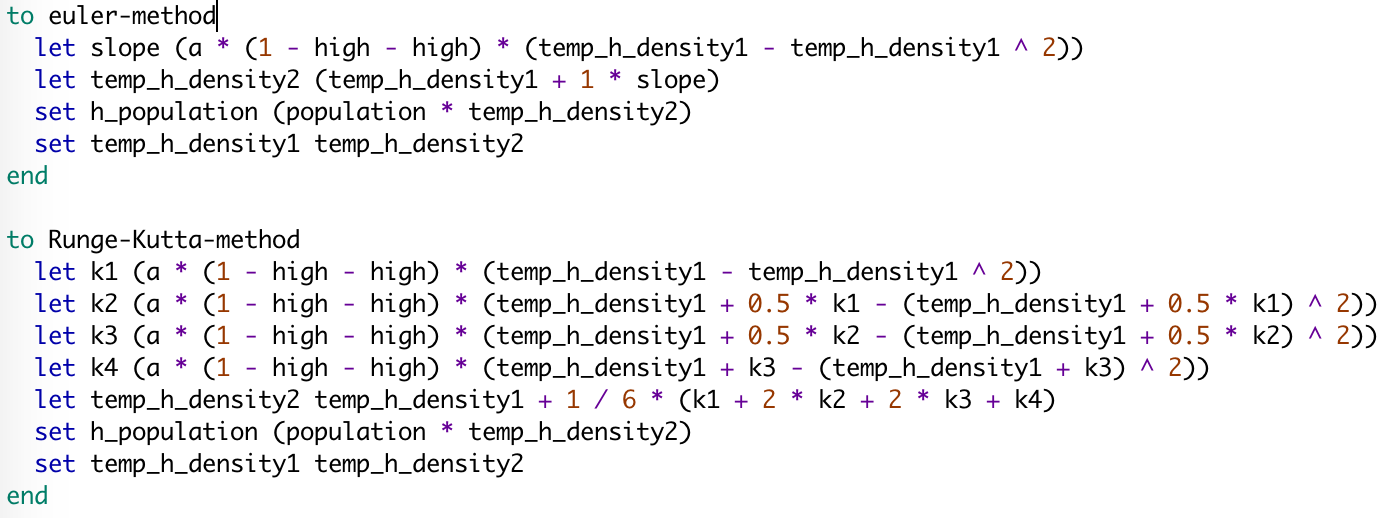
\includegraphics[width=6in]{./figures/code}
  \vspace{-3mm}
  \caption{\footnotesize Essential code for numerical integration}
  \label{integrate}
\end{figure}
\par The second part of the code above representing the 4th-level Runge-Kutta's method for numerical integration to solve this student dynamic systems.
\subsection{Comparison between analytical and numerical integration} 
As it shown below in figure 2, when using Euler's method there are some slightly error in the middle, however for the Runge–Kutta method it shows perfect match with the analytical integration.
\par As an evidence for the analyses of system behavior result, the figure below shows even if we changed the initial density for $H$ to be bigger than L, when $H>L$ ,the L will eventually dominate the population. 
\begin{figure}[!h]
  \centering
  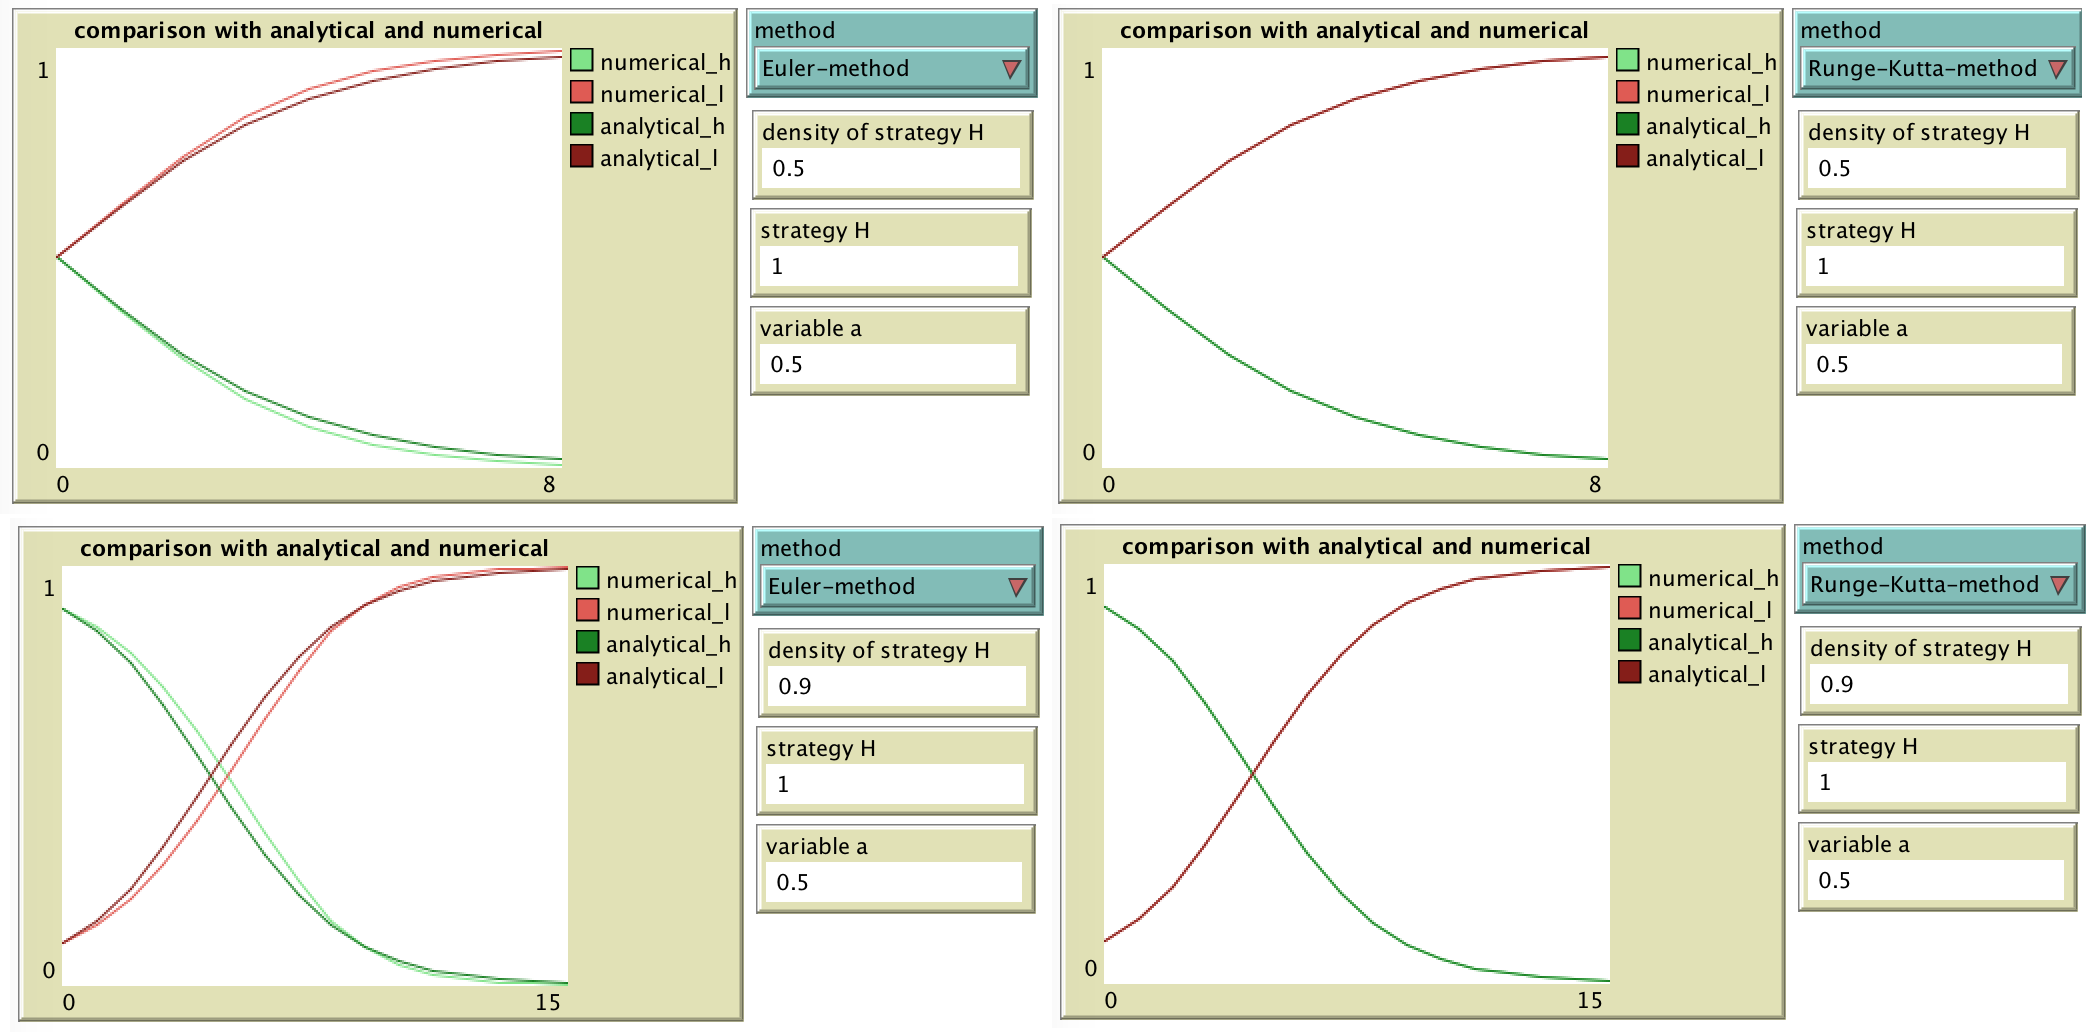
\includegraphics[width=6in]{./figures/comp}
  \vspace{-1mm}
  \caption{\footnotesize comparisons between integration methods}
  \label{comparison}
\end{figure}
\vspace{-3mm}

\subsection{Agent-based Model}
An agent-based model has been implemented based on Netlogo open source software to solve the same problem as described in section 1. 
\begin{itemize}[nolistsep]
	\item The agent world shown as the black area can display the group and regroup action after each course. 
	\item Population in each group is randomly distributed based on the groupnumber and the whole population, it is shown as a histogram on the left side.
\end{itemize}

\begin{figure}[!h]
\centering
	\begin{minipage}[t]{0.6\textwidth}
		\centering
		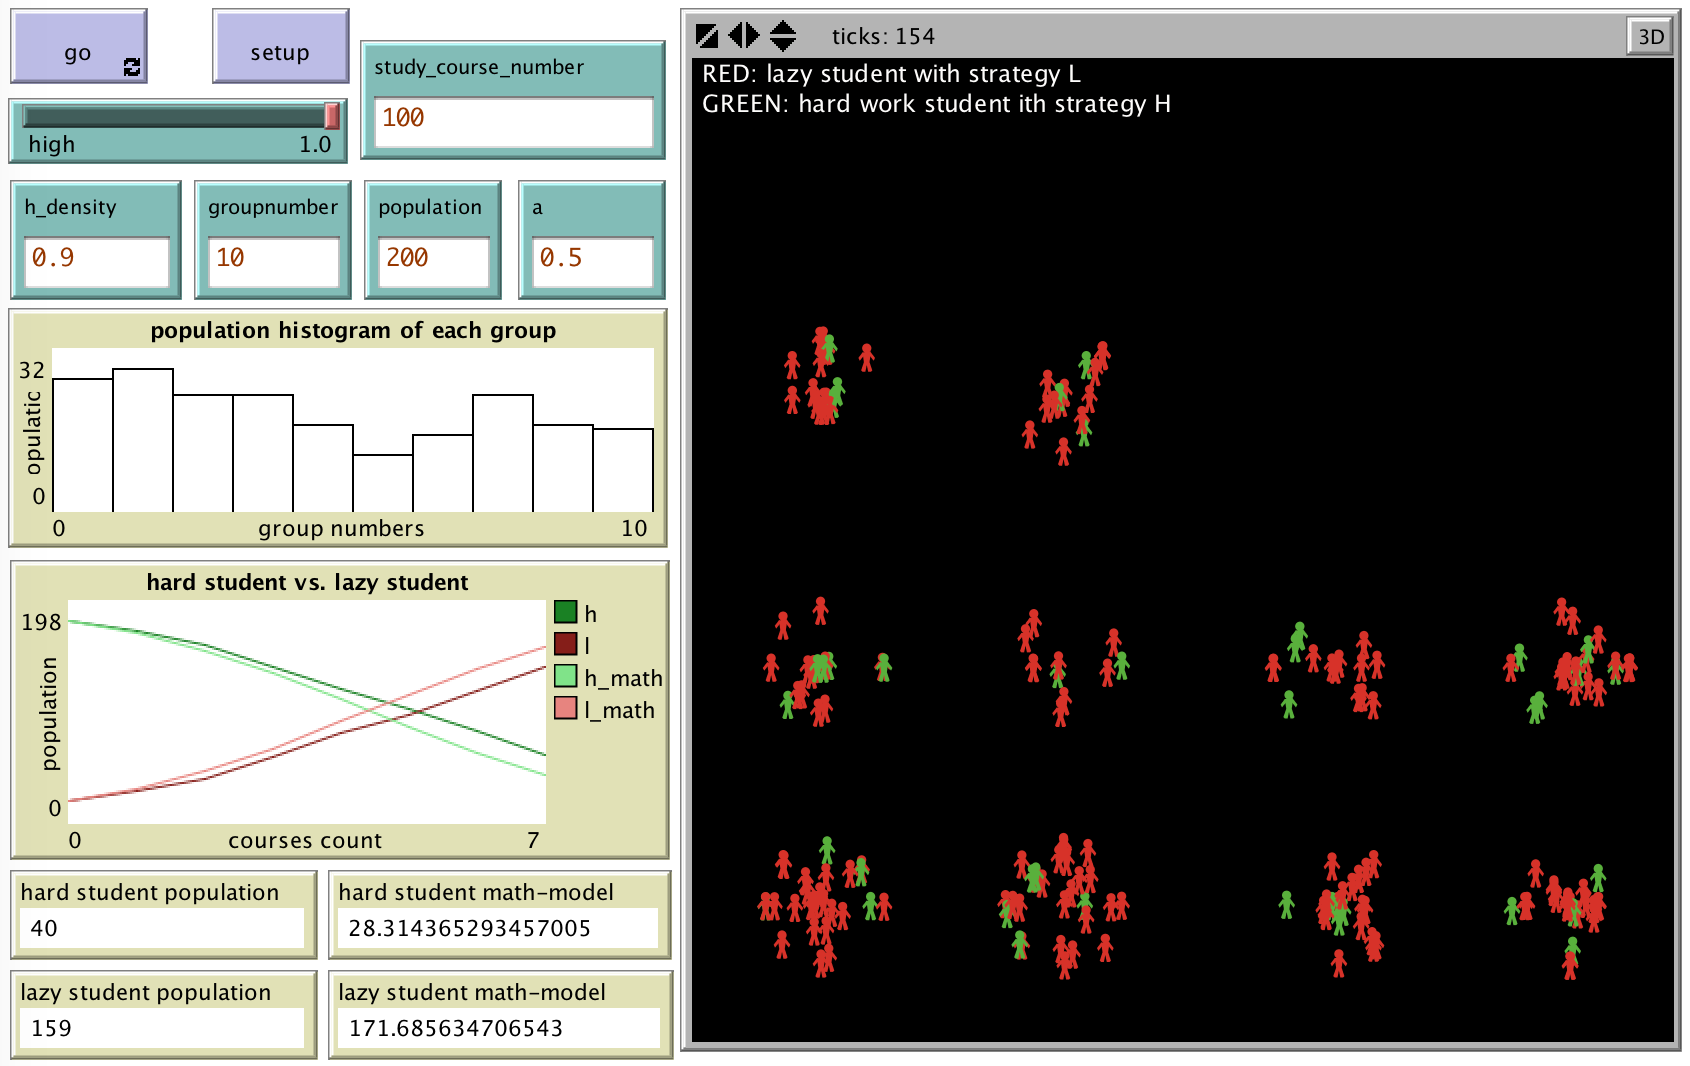
\includegraphics[width=1\linewidth]{./figures/agent}
		\begin{small}
			\centering
			\vspace{-6mm}
			\caption{\footnotesize Agent-based model}
		\end{small}
		\label{fig1}
	\end{minipage}
	\begin{minipage}[t]{0.25\textwidth}
		\centering
		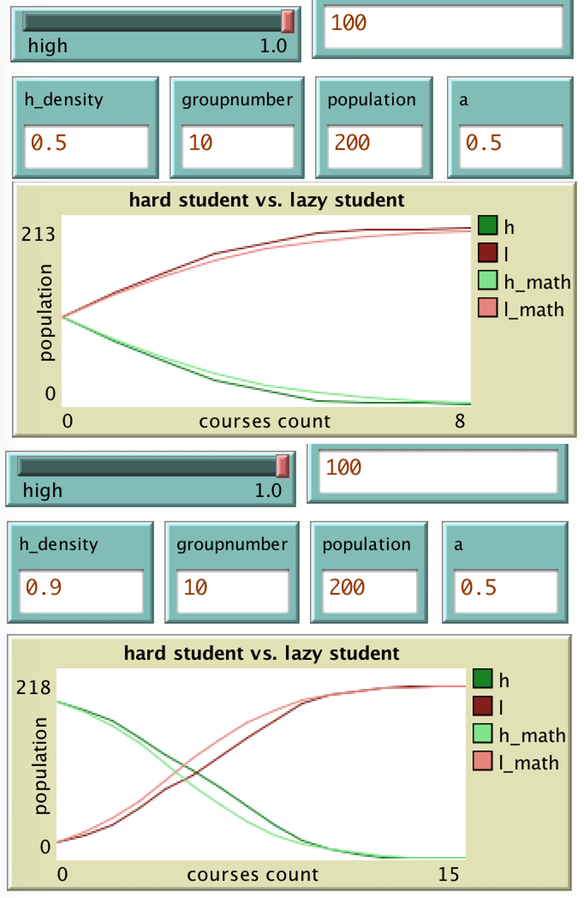
\includegraphics[width=1\linewidth]{./figures/agent-comp}
		\begin{small}
			\centering
			\vspace{-6mm}
			\caption{\footnotesize Comparison}
		\end{small}
		\label{fig2}
	\end{minipage}
\end{figure}
\vspace{-3mm}
\subsection{Comparison between integration and agent-based model}
This section describe the comparison of the system behavior between the numerical integration model and agent-based model. As a more accurate method, we use Runge-Kutta’s method for integration.

\section{Answer Research Questions}
Assume if we have equal numbers of hard working student and lazy student (H density = 0.5), the H = 1, L = 0 and a = 0.5. After 8 courses, the composition of each group will be \textbf{all lazy students} as it shown in figure 3. It will not change if we keep taking courses. Therefore, it takes 8 courses for this condition of the system to reach equilibrium state. 
\subsection{Evaluate each parameter}
\begin{itemize}[nolistsep]
	\item \textbf{Initial composition of the population (H density)}. As it shown in figure 3, if we only increase the population of hard working student in the beginning, it will take longer time to converge.
	\item \textbf{Group size}. The group size is determined by the groupnumber, for the example below, 50 
	groupnumbers means group size 4. It can be concluded that big group size can lead to quicker convergence. However it does not work when along with small a as shown in figure 4-4 and 4-5.
		\begin{figure}[!h]
		\centering
		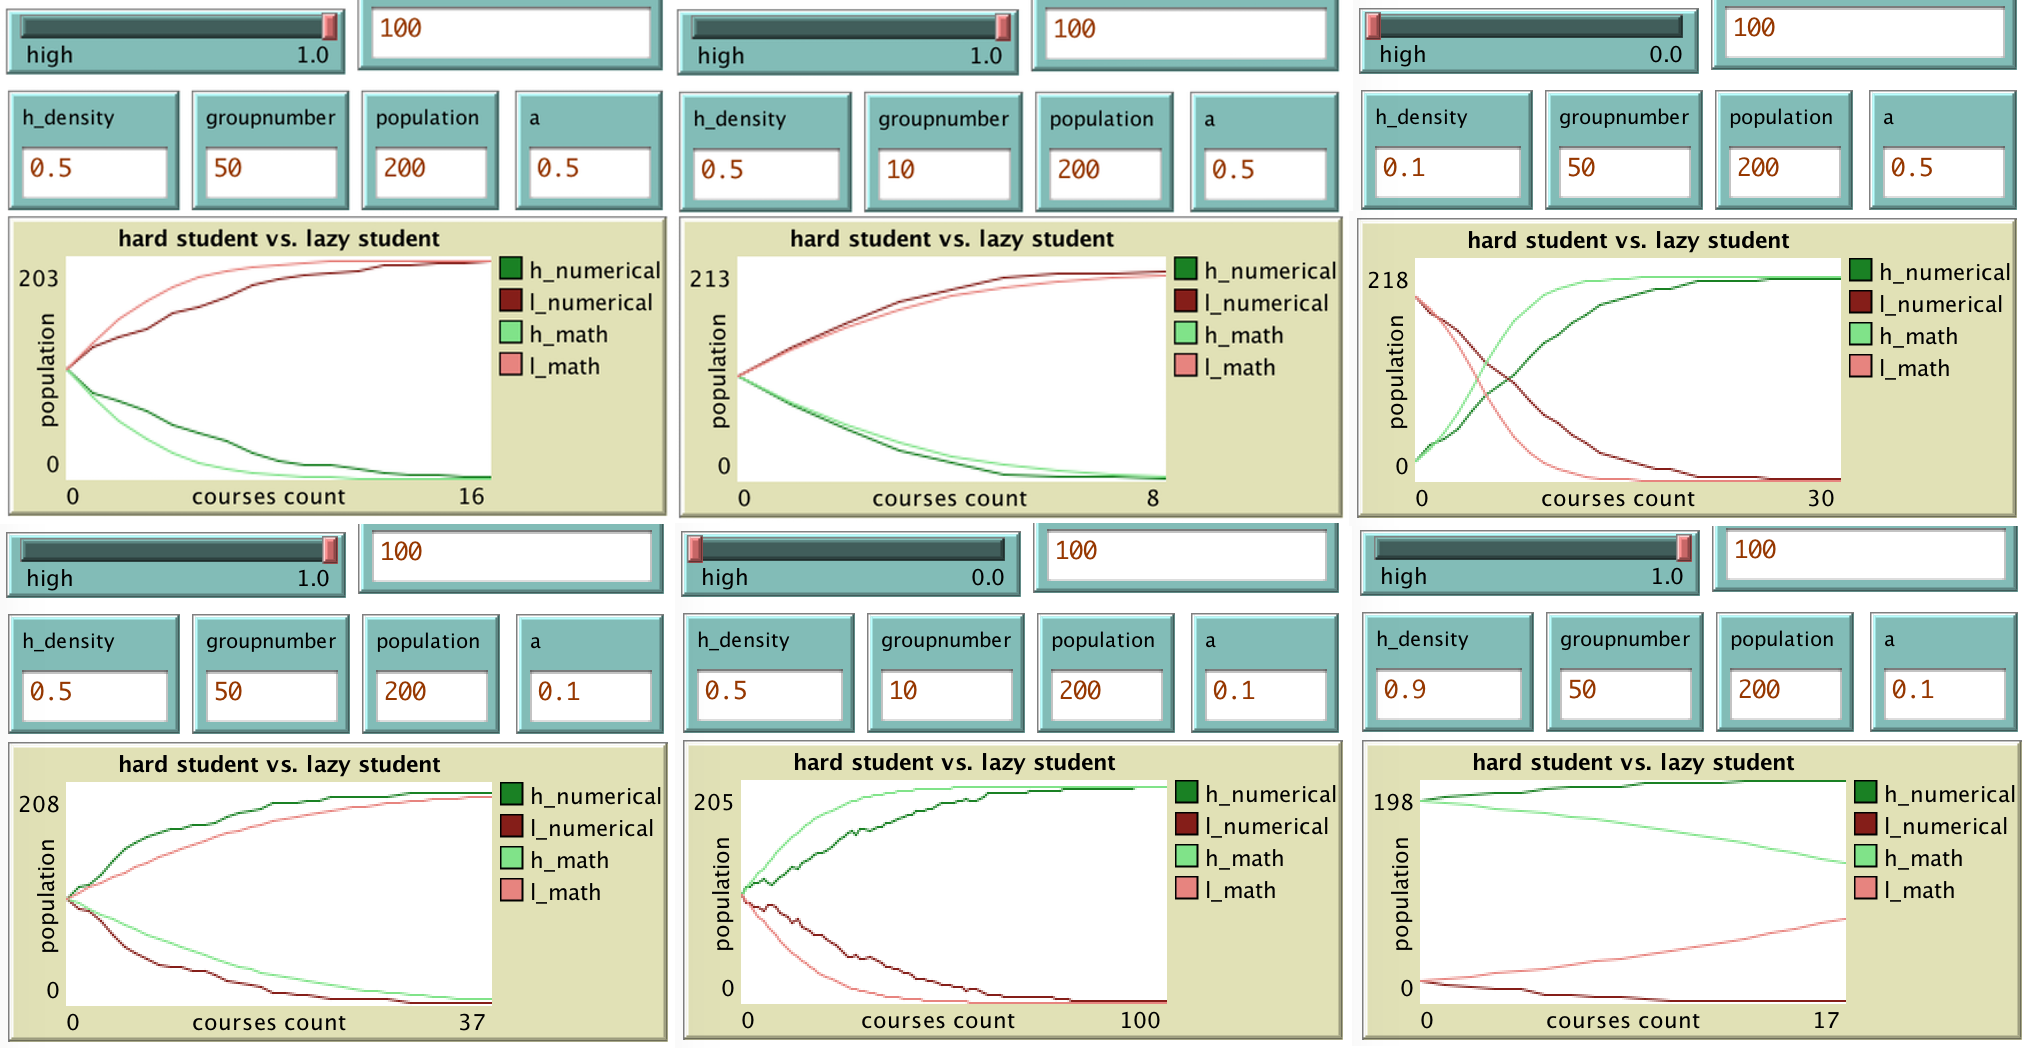
\includegraphics[width=6.5in]{./figures/all-comp}
		\vspace{-6mm}
		\caption{\footnotesize comparisons between different parameters}
		\label{comparison}
		\end{figure}
		\vspace{-3mm}
	\item \textbf{Cost of effort a}. Normally, smaller $a$ will cause slower convergence, special condition happen as described later.	
	\item \textbf{Strategy H and L}. It will determine the final result as analyzed in section 2.3, unless the a and group size fulfill the condition below. 
	\item \textbf{Small a with small group size}. If small a comes along with small group size it can cause the result to go completely opposite compare to numerical solution (figure 4-4 and 4-6).
\end{itemize}
\end{document}